\chapter{Implementierung}

\section{Grundlengende Implementierung}

Programmiersprachen: C und OpenCL\newline
Plattform: Darwin\newline
\newline
Wie bei Implementierungen mittels OpenCL �blich gliedert sich die Ausf�hrung in einen Host- und einen Target-Teil. Der Host-Teil wird wie gewohnt auf der CPU kompiliert und dann ausgef�hrt. Der Target-Code, welcher in OpenCL geschrieben ist, wird zur Laufzeit kompiliert, und dann auf das OpenCL-Device geladen und ausgef�hrt. OpenCL-Devices k�nnen sowohl CPUs als auch GPUs sein. In unserem Fall beschr�nken wir uns auf die parallele Ausf�hrung auf der GPU. Es steht uns eine Nvidia 9400M GPU zur Verf�gung, welche 16 Threads parallel ausf�hren kann. Die Implementierung unterst�tzt sowohl multithreading als auch multiple Devices (mehrere CPU-kerne oder mehre GPUs).
\newline
Der Host-Teil hat folgende Aufgaben:
\newline
\begin{itemize}
\item Initialisierung der Agenten
\item Kompilieren des OpenCL Codes
\item Allocation des OpenCL Devices
\item Kopieren der fixen Agenten in das Device Memory
\item Allocation von Target-Memory f�r bewegliche Agenten
\item Anstarten der OpenCL Execution
\item kopieren der beweglichen Agenten in das Host-Memory nach jeder Execution
\item generieren des Outputs in Form eines Bildes im ppm-format
\end{itemize}

Der Target-Teil hat folgende Aufgaben:

\begin{itemize}
\item Berechnung ob der dem thread zugewisene beweglicher Agent einen fixen Agent in Sichtweise hat
\item �nderung der aktuellen Bewegungsrichtung den Regeln folgend
\item Berechnung der neuen Position
\item Berechnung ob neue Position ausserhalb des Simulationsfeldes liegt. Wenn ja -> Abprall an der Wand.
\end{itemize}

Die Visualiserung der Simulation findet in mehreren Stufen statt. In der Host-Applikation wird nach jedem Simulationsschritt ein Bild generiert das den aktuellen Zustand mittels farbkodierter Punkte in einem Bild darstellt. Dazu wird aufgrund der Einfachkeit das simple PPM Format verwendet. Nach der Simulation werden die erzeugten ppm Bilder in das PNG-Format umgewandelt und ein Film mit HUFYU Codierung erzeugt. Wichtig bei der Wahl der Formate ist eine verlustfreie Kompression, da sonst Agenten, welche als einzelne Pixel dargestellt werden, verloren gehen k�nnten. Diese Darstellungskette wird als bash-script mithilfe von ffmpeg f�r die Codierung umgesetzt welche sowohl Einzelbilder der Simulationsschritte erzeugt als auch das Video mit der gesamten Simualtion. 


\section{Details}

Wie in \ref{fig:basic_arch} beschrieben, wird in der hier verwendeten Implementierung der eigentliche Algorithmus auf der GPU ausgef�hrt. Es wurde darauf Wert gelegt eine m�glichst universelle und erweiterbare Implementierung zu realisieren mit dem Focus auf eine gute Skalierbarkeit. Da bei dieser Aufgabenstellung zu erwarten ist, dass der Aufwand des Speichermanagementes und Speicherkopieren um einiges Zeitaufwendiger ist als die eigentliche Berechnung der Simulation wurde darauf Wert gelegt alle Speicheroperationen m�glichst schnell abzuschliessen. D.h. es wurde f�r alle Agenten der generelle GPU-Speicher verwendet und auf eine Allocation der Streaming-Speicher verzichtet welche schneller sind, aber auf 32kB limitiert sind. Weiters w�re wie schon beschrieben dadurch ein h�herer Zeitaufwand beim Speichermanagement zu erwarten was den Vorteil des schnelleren Speichers wohl zunichte machen w�rde.

Generell ist anzumerken dass die Generierung des Outputs und das Anschliessende umkodieren der Ergebnisse nach bisherigen Erfahrungen um einiges mehr Zeit in Anspruch nimmt als die Simulation selbst. Auch bei �ber 500000 beweglichen Agenten ist dies noch der Fall. Sollten l�ngere Simulationsintervalle gew�nscht werden ist es wohl als erstes Empfehlenswert nur alle N Simulationsschritte eine Ausgabe durchzuf�hren. Wenn dies nicht m�glich ist bzw. ungew�nscht kann man sich �berlegen eine Speicheroptimierung durchzuf�hren. Auch eine h�here Anzahl an fixen Agenten sollte diese Entscheidung beg�nstigen.


\begin{figure}[htb]
	\centering
		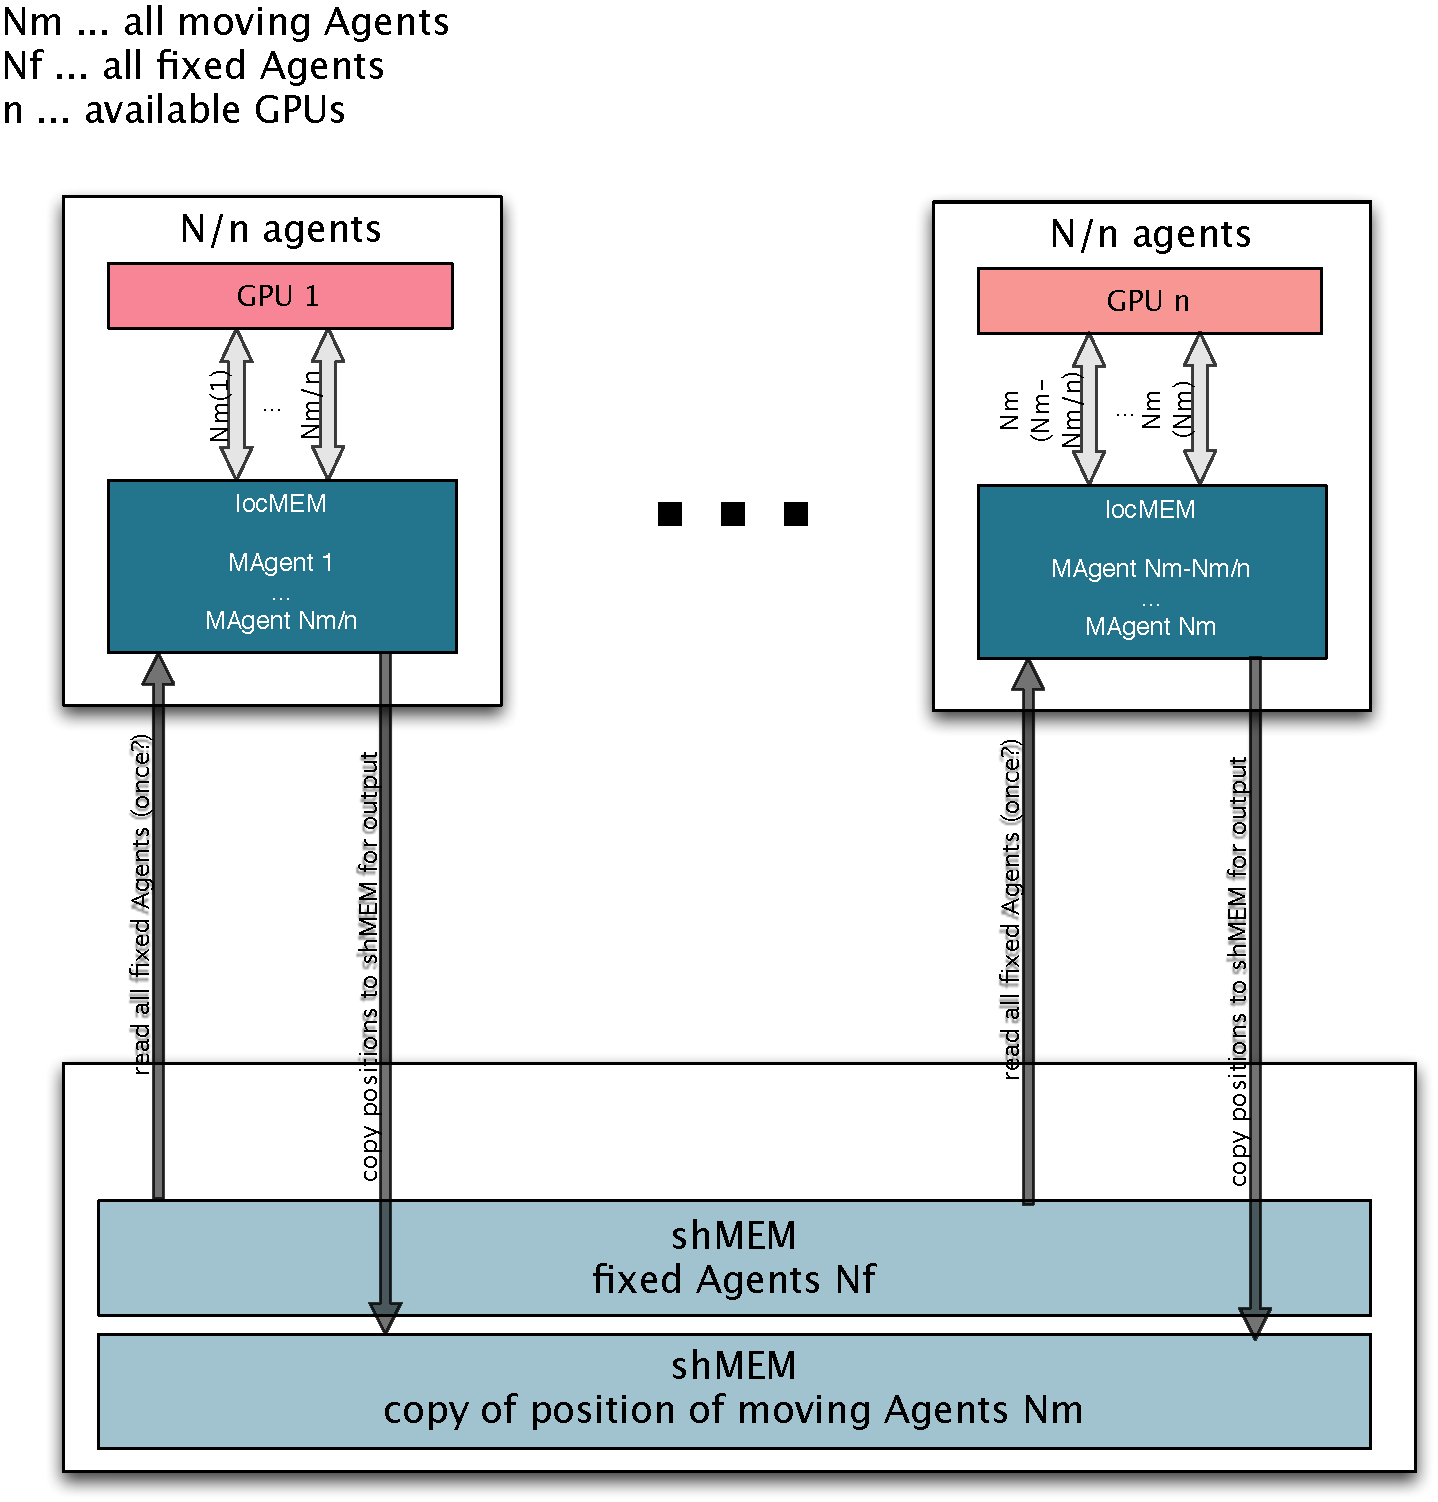
\includegraphics[width=1.0\textwidth]{chapter1/architecture.pdf}
	\caption{Basic Architecture}
	\label{fig:basic_arch}
\end{figure}
